\documentclass[10pt]{amsart}

\usepackage{macros,slashed}

\linespread{1.25}

\usepackage{tikz}
\usetikzlibrary{arrows,shapes}
\usetikzlibrary{trees}
\usetikzlibrary{matrix,arrows}
\usetikzlibrary{positioning}
\usetikzlibrary{calc,through}
\usetikzlibrary{decorations.pathreplacing}
\usepackage{pgffor}

\def\sAd{\sA{\rm d}}

\usetikzlibrary{decorations.pathmorphing}
\usetikzlibrary{decorations.markings}
\tikzset{
	% >=stealth', %%  Uncomment for more conventional arrows
    vector/.style={decorate, decoration={snake}, draw},
	provector/.style={decorate, decoration={snake,amplitude=2.5pt}, draw},
	antivector/.style={decorate, decoration={snake,amplitude=-2.5pt}, draw},
    fermion/.style={draw=black, postaction={decorate},
        decoration={markings,mark=at position .55 with {\arrow[draw=black]{>}}}},
    fermionbar/.style={draw=black, postaction={decorate},
        decoration={markings,mark=at position .55 with {\arrow[draw=black]{<}}}},
    fermionnoarrow/.style={draw=black},
    gluon/.style={decorate, draw=black,
        decoration={coil,amplitude=4pt, segment length=5pt}},
    scalar/.style={dashed,draw=black, postaction={decorate},
        decoration={markings,mark=at position .55 with {\arrow[draw=black]{>}}}},
    scalarbar/.style={dashed,draw=black, postaction={decorate},
        dwecoration={markings,mark=at position .55 with {\arrow[draw=black]{<}}}},
    scalarnoarrow/.style={dashed,draw=black},
    electron/.style={draw=black, postaction={decorate},
        decoration={markings,mark=at position .55 with {\arrow[draw=black]{>}}}},
	bigvector/.style={decorate, decoration={snake,amplitude=4pt}, draw},
}

\usepackage[final]{pdfpages}

\title{}

\def\opp{{\rm op}}
\def\Ch{{\rm Ch}}
\def\dgLie{{\rm dgLie}}
\def\Lcat{L_\infty{\rm Alg}}
\def\Cur{{\rm Cur}}

\def\brian{\textcolor{blue}{BW: }\textcolor{blue}}


\begin{document}
\maketitle
\tableofcontents

\section{The holomorphic charge anomaly}

For any BV theory $\sE$, the BV operator $\{S,-\}$, which satisfies $\{S,-\}^2 =0$ by the ordinary classical master equation, together with the BV bracket $\{-,-\}$ equip the space of local functionals $\oloc(\sE)$ with the structure of a dg Lie algebra. 
Another way to interpret the equivariant classical master equation is to view $I^{\sL}$ as an element in the dg Lie algebra $\oloc(\sE) \tensor \cloc^*(\sL)$.

This section is mostly a cobbling together of know results above BV quantization for holomorphic theories found in the sources \cite{CG2, BWhol}. 


%\subsection{The quantum master equation} 

Suppose that $\fg$ is an ordinary Lie algebra that exists as a symmetry of a particular classical field theory. 

\subsection{Equivariant holomorphic matter}

We introduce a classical field theory in the BV formalism that one may think of as higher dimensional ``matter" in a holomorphic setting. 
When the complex dimension is one this returns the chiral $\beta\gamma$ system from ordinary conformal field theory. 
In higher dimensions one can also realize this theory as a certain twist of supersymmetric matter. 
First, we motivate in terms of ordinary fields and \brian{not sure}. 

To start, we fix a finite dimensional $\fg$-module $V$ and an integer $d > 0$.
The classical fields of the complex $d$-dimensional theory consist of a map
\beqn\label{gammafield}
\gamma : \CC^d \to V
\eeqn
and a differential form of Hodge type $(d,d-1)$, $\beta \in \Omega^{d,d-1}(\CC^d, V^\vee)$ valued in the dual space $V^\vee$. 
The action functional describing the classical field theory is of the usual form
\beqn\label{actionfnl}
S(\gamma,\beta) = \int \<\beta, \dbar\gamma\>_V
\eeqn
where $\<-,-\>_V$ denotes the natural pairing between $V$ and its dual. 
The classical equations of motion of this theory consist of those $(\gamma,\beta)$ that are holomorphic, namely $\dbar \beta = \dbar \gamma = 0$. 

The gauge symmetry we consider comes from the $\fg$-action on $V$. 
This extends, in a natural way, to an action of the gauge Lie algebra $C^\infty(\CC^d, \fg)$ on the fields (\ref{gammafield}): an element $X(z,\zbar) \in C^\infty(X,\fg)$ acts simply by $X(z,\zbar) \cdot \gamma(z,\zbar)$ where the dot indicates product of functions and the $\fg$-module structure on $V$. 
The condition that this action be compatible with the action functional (\ref{actionfnl}) says precisely that $X(z,\zbar)$ must be holomorphic: $\dbar X(z,\zbar) = 0$. 

When $d=1$ to formulate this theory in the BV formalism we simply...\brian{finish}

\begin{dfn/lem}
The $\sG_d$-equivariant $\beta\gamma$ system on $\CC^d$ with values in $V$ is defined by the local functional
\[
I^{\sG}(\alpha, \beta, \gamma) = \int \<\beta, \alpha \cdot \gamma\>_V \in \oloc(\sE_V \oplus \sG_d[1]) .
\]
This functional satisfies the $\sG_d$-equivariant classical master equation
\[
(\dbar + \d_{\sG}) I^{\sG} + \frac{1}{2} \{I^{\sG}, I^{\sG}\} = 0 .
\] 
\end{dfn/lem}

\subsubsection{The $\beta\gamma$ factorization algebra}

It is the general philosophy of \cite{CG1,CG2} that the observables of a quantum field theory form a factorization algebra on the underlying spacetime. 

%In this section we describe the factorization algebra associated to the higher $\beta\gamma$ system on $\CC^d$ associated to any $\fg$-representation $V$. 

%For any vector space $W$, we can consider the commutative algebra of algebraic and formal algebraic functions denoted respectively by
%\[
%\sO(W) = \Sym (W^\vee) = \bigoplus_{n \geq 0} (W^\vee)^{\tensor n}_{S_n} \;\;\; , \;\;\; \Hat{\sO}(W) = \Hat{\rm Sym}(W^\vee) %= \prod_{n \geq 0} (W^\vee)^{\tensor n}_{S_n} . 
%\] 

For any theory, the factorization algebra of classical observables assigns to every open set $U$ the cochain complex of algebraic functions on the fields supported on $U$.  
For the example of the $\beta\gamma$ system, the differential is just given by the $\dbar$ operator. 
Concretely, the complex of classical observables\footnote{There is also the completed version where one uses $\prod$ in place of $\oplus$ when defining the symmetric algebra, but we will not use it here.} assigned to an open set $U$ is
\[
\Obs^{\cl}_V(U) = \left(\Sym \left(\Omega^{0,*}(U)^\vee \tensor V^\vee \oplus \Omega^{d,*}(U)^\vee \tensor V [-d+1]\right), \dbar\right) .
\]
As usual, we use the completed tensor product when defining the symmetric products. 
It follows from the general results of Chapter 6 of \cite{CG2} that this assignment defines a factorization algebra on $\CC^d$. 

Upon taking global sections, the functional $I^{\sG}$ defines a map of dg Lie algebras $I^{\sG} : \sG_d(\CC^d) \to \Obs^{\cl}_V(\CC^d)$.
We have seen that $\Obs_V^{\cl}$ is a factorization algebra equipped with a $P_0$-structure. 
In the introduction, we also discussed how a local Lie algebra determines a $P_0$-factorization algebra via its classical current algebra. 
The classical Noether's theorem, as proved in Chapter 11 of \cite{CG2}, says that $I^{\sG}$ determines a map between these factorization algebras. 

\begin{prop}{\cite{[CG2]}} (Classical Noether's Theorem)
The assignment that sends an element $\alpha \in \Omega^{0,*}_c(U, \fg)$ to the observable
\[
\gamma \tensor \beta \in \Omega^{0,*}(U, V) \tensor \Omega^{d,*}(U, V^*) \mapsto \int_U \<\beta, \alpha \cdot \gamma\>_V
\]
determines a map of $P_0$-factorization algebras on $\CC^d$
\[
J^{\cl} : \Cur^{\cl} (\sG_d) \to \Obs^{\cl}_V .
\]
\end{prop}

\begin{rmk}
The formula for $J^{\cl}$ is identical to that of the local functional $I^\fg(\alpha)$ defining the action of $\sG_d$ on the $\beta\gamma$ system.
Ordinarily, a local functional does not determine an observable on an open set since the integral may not exist.
However, since $\alpha$ is compactly supported on $U$, it makes sense to restrict $I^\sG (\alpha)$ to an observable on $U$. 
This is precisely the observable $J^{\cl}(\alpha)$. 
\end{rmk}

As always, the statement we are after pertains to the quantum situation. 
Being a free field theory, the $\beta\gamma$ system admits a unique quantization and hence a factorization algebra $\Obs^{\q}_V$ of quantum observables (whose definition we recall below). 
The natural question arises whether the symmetry by the dg Lie algebra $\sG_d$ persists upon quantization. 
We are asking if we can lift $J^{\cl}$ to a ``quantum current" $J^{\q} : \Cur^\q(\sG_d) \to \Obs^\q_V$, where $\Cur^\q(\sG_d)$ is the factorization algebras of quantum currents defined in the introduction. 
The existence of this map of factorization algebras is controlled by the equivariant quantum master equation, which we now turn to.

\subsection{The quantization}

The approach to quantum field theory we use follows Costello's theory of renormalization and the Batalin-Vilkovisky formalism developed in \cite{CosRenorm}.
The formalism dictates that in order to define a quantization, it suffices to define the theory at each energy (or length) scale and to ask that these descriptions be compatible as we vary the scale.
Concretely, this compatibility is through the {\em renormalization group (RG) flow} and is encoded by an operator $W(P_{\epsilon < L}, -)$ acting on the space of functionals. 
The functional $W(P_{\epsilon < L},-)$ is defined as a sum over weights of graphs which is how Feynman diagrams appear in Costello's formalism.
The quantization we work with follows this general approach very closely, with the slight caveat that we are working equivariantly, and so some of the fields are actually background fields. 

The two main ingredients to construct the weight are the propagator $P_{\epsilon < L}$ and the classical interaction $I^{\sG}$. 
The propagator only depends on the underlying free theory, that is, the higher dimensional $\beta\gamma$ system. 
As above, the interaction describes how the linear currents $\sG_d$ act on the free theory. 

Our definition of the propagator $P_{\epsilon<L}$ follows the general approach given in Section ?? of \cite{CG2}.
The construction of $P_{\epsilon<L}$, which makes sense for a wide class theories of this holomorphic flavor, can be found in Section 3.2 of \cite{BWhol}.
For us, it is important to know that $P_{\epsilon<L}$ satisfies the following properties:
\begin{enumerate}
\item[(1)] For $0 < \epsilon < L < \infty$ the propagator is a symmetric element
\[
P_{\epsilon < L} \in \sE_V \Hat{\tensor} \sE_V .
\]
Moreover, $P_{0 < \infty} = \lim_{\epsilon \to 0}\lim_{L \to \infty}$ is a symmetric element of the distributional completion $\Bar{\sE}_V \Hat{\tensor} \Bar{\sE}_V$. 

\item[(2)] 
The propagator lies in the subspace
\[
\Omega^{d,*}(\CC^d \times \CC^d, V \tensor V^*) \oplus \Omega^{d,*}(\CC^d \times \CC^d, V^* \tensor V) \subset \sE_V \Hat{\tensor} \sE_V .
\]
If we coordinatize $(z,w) \in \CC^d \times \CC^d$, the propagator has the form
\beqn
P_{\epsilon<L} = P^{an}_{\epsilon<L}(z,w) \tensor \left({\rm id}_{V} + {\rm id}_{V^*}\right)
\eeqn
where ${\rm id}_V, {\rm id}_{V^*}$ are the elements representing the identity maps which lie in $V \tensor V^*, V^* \tensor V$ respectively. 
Moreover, $P^{an}_{0 < \infty} (z,w)$ is the Green's function for the Hodge Laplacian $\triangle_{\rm Hodge}$ on $\CC^d$:
\[
\triangle_{\rm Hodge} P^{an}_{0<\infty} (z,w) = \delta (z-w) .
\]

\item[(3)] Let $K_t \in C^\infty((0,\infty)_t) \tensor \sE_V \Hat{\tensor} \sE_V$ be the heat kernel for the Hodge Laplacian
\[
\triangle_{\rm Hodge} K_t + \frac{\partial}{\partial t} K_t = 0 .
\]
Then, $P_{\epsilon < L}$ provides a $\dbar$-homotopy between $K_\epsilon$ and $K_L$:
\[
\dbar P_{\epsilon < L} = K_{t=L} - K_{t=\epsilon} .
\]
\end{enumerate}

%The building block in Costello's approach to renormalization is an effective family of functionals $\{I[L]\}$ parametrized by a {\em length scale} $L > 0$. 
%For each $L > 0$ the functional $I[L] \in \sO(\sE)[[\hbar]]$ must satisfy various conditions, which are carefully stated in Definition 8.2.9.1 of \cite{CG2}. 
%We will recall some key aspects that will be useful for our purposes. 
%The main condition is a compatibility between the functionals $I[L]$ as one changes the length scale; this is referred to as {\em homotopy renormalization group (RG) flow}.

To define the quantization, we must recall the definition of a weight of a Feynman diagram adjusted to this equivariant context.
To simplify our discussion, we introduce the notation $\sO(\sG_d[1])$ to mean the underlying graded vector space of $\clie^*(\sG_d)$, so the symmetric algebra on the dual of $\sG_d$. 

For the free $\beta\gamma$ system, the homotopy RG flow from scale $L>0$ to $L'>0$ is an invertible linear map 
\beqn\label{weight1}
W(P_{L < L'} , -) : \sO(\sE) [[\hbar]] \to \sO(\sE)[[\hbar]]
\eeqn
defined as a sum over weights of graphs $W (P_{L<L'}, I) = \sum_{\Gamma} W_{\Gamma}(P_{L<L'}, I)$. 
Here, $\Gamma$ denotes a graph, and the weight $W_\Gamma$ associated to $\Gamma$ is defined as follows.
One labels the vertices of valence $k$ by the $k$th homogenous component of the functional $I$. 
The edges of the graph are labeled by the propagator $P_{L<L'}$.
The total weight is given by iterative contractions of the homogenous components of the interaction with the propagator. 
Formally, we can write the weight as
\[
e^{W(P_{\epsilon <L}, I)} = e^{\hbar \partial_{P_{\epsilon <L}}} e^{I / \hbar}
\]
where $\partial_P$ denotes contraction with $P$. 
For a more precise definition see Chapter 2 of \cite{CosRenorm}.

To define the equivariant version, we extend (\ref{weight1}) to a $\sO(\sG_d[1])$-linear map
\[
W^{\sG} (P_{L < L'} , -) : \sO(\sE \oplus \sG_d[1]) [[\hbar]] \to \sO(\sE \oplus \sG_d[1])[[\hbar]] .
\]
Introduce the weight $W(P_{\epsilon < L}, I^{\sG})$
\begin{dfn/lem}
The prequantization of the $\sG_d$-equivariant $\beta\gamma$ system on $\CC^d$ is defined by the family of functionals $\{I^{\sG}[L]\}_{L > 0}$ where
\beqn\label{prequant}
I^{\sG} [L] = \lim_{\epsilon \to 0} W^{\sG} (P_{\epsilon<L} , I^{\sG}) .
\eeqn 
This family satisfies homotopy RG flow and solves the quantum master equation modulo $\cloc^*(\sG_d)$. 
\end{dfn/lem}

\begin{proof}
The non-trivial claim to justify here is why the $\epsilon \to 0$ limit of $W^{\sG} (P_{\epsilon<L} , I^{\sG})$ exists. 
This follows from the following two claims:

\begin{itemize}
\item[(1)] 
Only one-loop graphs appear in the weight expansion $W^{\sG} (P_{\epsilon < L}, I^{\sG})$. 

\item[(2)] Let $\Gamma$ be a one-loop graph.
Then
\[
\lim_{\epsilon \to 0} W^{\sG}_\Gamma(P_{\epsilon < L}, I^{\sG})
\]
exists.
\end{itemize}

First, we justify claim (1).
Recall that the weight is defined as a sum over {\em connected} graphs.
An immediate consequence of the combinatorics involved in constructing the equivariant weight using the $\beta\gamma$ propagator \brian{finish}. 



\end{proof}



\begin{lem}
For each $L > 0$, the functional $I^{\sG}[L]$ lies in the subspace $\sO(\sE \oplus \sG_d[1]) [\hbar] \subset \sO(\sE \oplus \sG_d[1]) [[\hbar]]$. 
\end{lem}

To define the quantum master equation, we must introduce the BV Laplacian $\Delta_L$ and the scale $L$ BV bracket $\{-,-\}_L$. 
For $L > 0$, the operator $\Delta_L : \sO(\sE_V) \to \sO(\sE_V)$ is defined by contraction with the heat kernel $K_L$ defined above. 
Similarly, $\{-,-\}_L$ is defined by \brian{equation}. 
There are equivariant version of each of these operators by extending via $\sO(\sG_d[1])$-linearity.
For instance, the BV Laplacian is a degree one operator of the form
\[
\Delta_L : \sO(\sE \oplus \sG_d[1]) \to \sO(\sE \oplus \sG_d[1]) .
\]
We say a functional $J \in \sO(\sE_V \oplus \sG_d[1])$ satisfies the scale $L$, $\sG_d$-equivariant quantum master equation if
\[
(\dbar + \d_{\sG}) J+ \frac{1}{2} \{J, J\}_L + \hbar \Delta J = 0 .
\]
The main object of study in this section is the failure for the quantization $I^{\sG}[L]$ to satisfy this equivariant QME. 

\begin{dfn}
The scale $L$, $\sG_d$-equivariant charge anomaly is
\[
\hbar \Theta_V [L] = (\dbar + \d_{\sG}) I^{\sG} [L] + \frac{1}{2} \{I^{\sG}[L], I^{\sG}\}_L + \hbar \Delta I^{\sG}[L] .
\]
As above, $\d_{\sG}$ denotes the Chevalley-Eilenberg differential $\clie^*(\sG_d) = \left(\sO(\sG_d[1]), \d_{\sG}\right)$. 
\end{dfn}

\subsection{The charge anomaly for $\beta\gamma$}

To calculate the anomaly to solving the $\sG_d$-equivariant master equation we utilize a general result about the quantum master equation for holomorphic field theories formulated in \cite{BWhol}. 
In general, since the effective field theory defining the prequantization $\{I^{\sG}[L]\}$ is given by a Feynman diagram expansion, the anomaly to solving the quantum master equation is also given by a potentially complicated sum of diagrams. 
As an immediate corollary of Proposition 4.4 for holomorphic theories on $\CC^d$, we find that only a simple class of diagrams appear in the anomaly. 

\begin{lem}\label{lem: obs}
Let $\Theta[L]$ be the obstruction to solving the $\sG_d$-equivariant quantum master equation.
Then, $\Theta := \lim_{L \to 0} \Theta[L]$ exists, and is a local cocycle 
\[
\Theta \in \cloc^*(\sG_d) .
\]
Furthermore, $\Theta$ is computed by the following limit
\[
\hbar \Theta = \frac{1}{2} \lim_{L \to 0} \lim_{\epsilon \to 0} \sum_{\Gamma \in {\rm Wheel}_{d+1} \; , e} W_{\Gamma, e}(P_{\epsilon <L}, K_\epsilon, I^{\sG}) ,
\] 
where the sum is over all wheels of valency $(d+1)$ and internal edges $e$. 
\end{lem}

\begin{rmk}
If $\Gamma$ is a graph with a distinguished edge $e$ and $A,B$ are elements of the tensor square of fields $A, B \in \sE \tensor \sE$, we let $W_{\Gamma,e}(A,B, I)$ denotes the weight of the graph where we place $B$ at the internal edge labeled $e$ and $A$ on the remaining internal edges.
\end{rmk}

In the remainder of this section we will characterize this anomaly algebraically, using the identification of Proposition \cite{prop: trans j}. 
Actually, it is immediate based on symmetry arguments what the obstruction is up to a scalar multiple. 

First, we note that the element $\Theta \in \cloc^*(\sG_d)$ lifts to the invariant subspace of $U(d)$-invariant, holomorphic translation invariant local cocycles.
This follows from the fact that both the functional $I^{\sG}$ and propagator $P_{\epsilon<L}$ are $U(d)$-invariant, holomorphic translation invariant.
By Proposition \ref{prop: trans j} we see that $\Theta$ must be cohomological to a cocycle of the form
\[
(\alpha_0, \ldots, \alpha_d) \mapsto \int_{\CC^d} \theta(\alpha_0 \wedge \partial \alpha_1 \wedge \cdots \wedge \partial \alpha_d) 
\]
where $\theta$ is some element of $\Sym^{d+1}(\fg^*)^\fg$.
In the notation of Section \ref{??}, this is the cocycle $\fJ_d (\theta)$. 
This cocycle factors in the following way:
\beqn\label{composition}
\begin{tikzcd}
\left(\Omega^{0,*}_c(\CC^d) \tensor \fg\right)^{\tensor (d+1)} \ar[r,"\fa \fn"] & \left(\Omega^{0,*}_c(\CC^d) \tensor \fg\right) \tensor \left(\Omega^{1,*}_c(\CC^d)\tensor \fg\right)^{\tensor d} \ar[r, "\theta"] & \Omega^{d, *}_c(\CC^d) \ar[r, "\int"] & \CC . 
\end{tikzcd}
\eeqn
The first map is $\fa \fn : \alpha_0 \tensor \cdots \tensor \alpha_d \mapsto \alpha_0 \tensor \partial \alpha_1 \tensor \cdots \tensor \partial \alpha_d$.
The second map is given by extending the Lie algebraic functional $\theta : \fg^{\tensor (d+1)} \to \CC$ to the Dolbeault complex in the obvious way:
\[
\theta \left(\alpha_0 \tensor (\alpha_1 \tensor \cdots \tensor \alpha_d\right) = \alpha_0 \wedge \theta(\alpha_1 \wedge \cdots \wedge \alpha_d) \in \Omega^{d,*}_c(\CC^d).
\]

Lemma \ref{lem: obs} implies that the obstruction is given by the sum over Feynman weights associated to graphs of wheels of valency $(d+1)$.
We can identify the algebraic component, corresponding to $\theta$ in the above composition (\ref{composition}), directly from the shape of this graph. 
The propagator and heat kernel $P_{\epsilon<L}, K_\epsilon$ labeling the edges factor as
\[
P_{\epsilon<L} = P^{an}_{\epsilon<L} \tensor \left({\rm id}_{V} + {\rm id}_{V^*}\right) \;\; , \;\; K_{\epsilon} = K_{\epsilon}^{an} \tensor \left({\rm id}_{V} + {\rm id}_{V^*}\right)
\]
where ${\rm id}_V, {\rm id}_{V^*}$ are the elements representing the identity maps which lie in $V \tensor V^*, V^* \tensor V$ respectively. 
The analytic factors $P^{an}_{\epsilon<L},  K_{\epsilon}^{an}$ only depend on the dimension $d$. 

Each trivalent vertex of the wheel is also labeled by both an analytic factor and Lie algebraic factor. 
The Lie algebraic part of each vertex can be thought of as the defining map of the representation $\rho : \fg \to {\rm End}(V)$. 
The diagrammatics of the wheel amounts to taking the trace of the symmetric $(d+1)$st power of this Lie algebra factor. 
Thus, the Lie algebraic factor of the weight of the wheel is the $(d+1)$st component of the character of the representation
\[
{\rm ch}_{d+1}^\fg(V) = \frac{1}{(d+1)!} {\rm Tr}\left(\rho(X)^{d+1}\right) \in \Sym^{d+1}(\fg^*) .
\]

By these symmetry arguments, we know that the anomaly will be of the form $\Theta = A \fj (\ch_{d+1}^{\fg}(V))$ for some number $A \in \CC$.
In Appendix \ref{sec: feynman}, we perform an explicit calculation of this constant $A$, which depend on the specific form of the analytic propagator and heat kernel. 

\begin{prop}\label{prop: bg anomaly}
The charge anomaly for quantizing the $\sG_d$-equivariant $\beta\gamma$ system on $\CC^d$ is equal to
\[
\Theta = A  \fj (\ch_{d+1}^{\fg}(V)),
\]
where $\fj$ is the isomorphism from Proposition \ref{prop: trans j}.
\end{prop}

\subsection{Free field realization}

The failure to satisfying the equivariant quantum master equation measures the obstruction to lifting the classical Noether map (\ref{cnoether}) to a map of factorization algebras from the quantum current algebra $\Cur^\q(\sG_d)$. 
The obstruction $\Theta$ to solving the quantum master equation implies that we have a map from the {\em twisted} quantum current algebra. 
As an immediate corollary of Theorem 12.1.0.2 \cite{CG2} we have the following. 

\begin{prop}
Let $\hbar \Theta_V$ be the obstruction to satisfying the $\sG_d$-equivariant quantum master equation. 
There is a map of factorization algebras on $\CC^d$ from the twisted quantum current algebra to the quantum observables
\beqn\label{qnoether}
J^\q : \Cur_{\hbar \Theta_V}^\q (\sG_d) \to \Obs^\q_V 
\eeqn
that fits into the diagram of factorization algebras
\[
\begin{tikzcd}
\Cur^\q_{\hbar \Theta_V} (\sG_d) \ar[d, "\hbar \to 0"'] \ar[r, "J^\q"] & \Obs^\q_V \ar[d, "\hbar \to 0"] \\
\Cur^\cl (\sG_d) \ar[r,"J^\cl"] & \Obs^{\cl}_V .
\end{tikzcd}
\]
\end{prop}

The quantum current algebra $\Cur^\q_{\hbar \Theta_V}$ is a factorization algebra on $\CC^d$ taking values in $\CC[\hbar]$. 
It therefore makes sense to specialize the value of $\hbar$. 
The convention we take is to specialize the value of $\hbar$ to be
\[
\hbar = (2\pi i)^d .
\]

From our calculation of the charge anomaly $\Theta_V$ above, once we specialize $\hbar$ we can realize the current algebra as an enveloping factorization algebra
\[
\left. \Cur^\q_{\hbar \Theta_V} (\sG_d) \right|_{\hbar = (2\pi i)^d} \cong \UU_{\ch_{d+1}^\fg(V)} (\sG_d) .
\]
Thus, as an immediate corollary of the above proposition, $J^\q$ specializes to a map of factorization algebras
\[
J^\q : \UU_{\ch_{d+1}^\fg(V)} (\sG_d) \to \left. \Obs^\q_V \right|_{\hbar = (2\pi i)^d} .
\]

\subsubsection{}

%\begin{cor}
%There is a map of factorization algebras on $\CC^d$, $\Phi^\q : \UU_{\# \ch_{d+1}(\fg^{ad})}(\fg^{\CC^d}) \to \Obs^\q_V$ 
%that fits into the following diagram 
%\[
%\begin{tikzcd}
% \UU_{\# \ch_{d+1}(\fg^{ad})} (\fg^{\CC^d}) \ar[d] \ar[r, dotted, "\Phi^\q"] & \Obs^\q_V \ar[d, "\hbar \to 0"] \\
% \UU (\fg^{\CC^d}) \ar[r, "\Phi^{cl}"] & \Obs^{cl}_V ,
% \end{tikzcd}
% \]
% where $\Phi^{cl}$ is as in Equation (\ref{classicalPhi}). 
% \end{cor}


%%%%%%%%%%%%%%%%%%%%%%%%%%%%% OLD DRAFT BELOW %%%%%%%%%%%%%%%%%%%%%

\appendix

\section{Calculation of the analytic weight} \label{sec: feynman}

\section{A very local Grothendieck-Riemann-Roch theorem}

The main goal of the BV formalism developed in \cite{CostelloRenormalization} is to rigorously construct quantum field theories using a combination of homological methods and a rigorous model for renormalization. 
A particular nicety of this approach is the ability to study {\em families} of field theories, which we will turn into an equivariant version of BV quantization, see Section \ref{sec: equiv BV}. 
In this section we will consider a family of QFT's parametrized by the moduli space of principal $G$-bundles. 
Our main result is to interpret a certain anomaly coming from BV quantization as a families index over ${\rm Bun}_G(X)$. 
This anomaly is computed via an explicit Feynman diagrammatic calculation and is related to a local cocycle of the current algebra discussed in Section \ref{sec: g j functional}.
 
We interpret this result as a formal universal version of the Grothendieck-Riemann-Roch theorem over the moduli space of bundles. 
The main idea is that the local cocycles we have just discussed in Section \ref{sec: g j functional} can be interpreted as characteristic classes on the (formal neighborhood) of the moduli space of $G$-bundles.

We will arrive at the result in a way that is local-to-global on spacetime which we formulate in terms of factorization algebras.
The main them of Costello and Gwilliam's approach to QFT is that the observables of a QFT determine a factorization algebra. 
We study the associated family of factorization algebras associated to the family of QFT's over the moduli space of $G$-bundles.
We will recollect a formulation of Noether's theorem for symmetries of a theory in terms of factorization algebras developed in Chapter 11 of \cite{CG2}. 
The central object in this discussion is a ``local index" which describes how the Kac-Moody factorization algebra acts on the observables of the QFT. 
Locally on spacetime we see how Noether's theorem provides a {\em free field realization} of the Kac-Moody factorization algebra generalizing that of the Kac-Moody vertex algebra in chiral conformal field theory \cite{FrenkelFree}. 

We now give a brief summary of the results, with a background for the situation we consider.
Suppose that $P$ is a fixed holomorphic $G$-bundle on a complex manifold $X$.
We have already seen how to express the formal deformation space of $P$ inside of the moduli of $G$-bundles using the dg Lie algebra $\sAd(P)(X) = \Omega^{0,*}(X , \ad (P))$.
In particular, any Maurer-Cartan element of $\sAd(P)(X)$ defines a deformation of $P$. 
We have seen that there is a refinement of this dg Lie algebra to a local Lie algebra $\sAd(P)$ whose factorization envelope defines the higher Kac-Moody factorization algebra above.
To any $G$-representation $V$ we will define a holomorphic theory with fields $\sE_V$ that is equivariant for this local Lie algebra. 
Equivalently, we can think of $\sE_V$ as defining a family of theories over the formal completion of $P$ in the moduli of $G$-bundles
\[
\xymatrix{
\sE_V|_{P'} \ar[d] \ar[r] & \sE_V \ar[d] \\
\{P'\} \ar[r] & {\rm Bun}_G(X)^{\wedge}_P .
}
\]
Over each fiber $P'$ the theory $\sE_V|_{P'}$ is a {\em free} theory, so admits a canonical BV quantization. 
Our formulation of equivariant BV quantization is codification of the problem of gluing together these quantizations in a compatible way.
We will show how this presents itself in the failure of the BV quantization to be a {\em flat} family. 
Our main result is the following. 

\begin{thm}\label{thm ggrr}
Let $P$ be any principal $G$-bundle over a compact affine complex manifold $X$ of dimension $d$.
Suppose   $V$ is a $G$-representation.
Then, the factorization homology $\int_X \Obs^\q_{V}$ defines a line bundle over the formal neighborhood of $P$ inside of the moduli of $G$-bundles.
Moreover, its first Chern class is 
\[
c_1\left(\int_X \Obs^\q_{V}\right) = C \ch_{d+1}^\fg (V)
\]
under the identification of $\ch_{d+1}^{\fg} (V)$ as a cohomology class on the formal neighborhood of $P$ inside of the moduli of $G$-bundles in Equation (\ref{cohbung}) explained below.
Here, $C$ is some nonzero complex number.
\end{thm}

There is an elucidating geometric description of how the classes $\ch_{d+1}(V)$ appear: they describe curvatures of line bundles over the moduli of $G$-bundles.
Let ${\rm Bun}_{G}(X)$ denote the moduli space of $G$-bundles on the complex $d$-fold $X$. \footnote{For $d > 1$ \cite{FHK} have constructed a global smooth derived realization of this space, but its full structure will not be used in this discussion.}
Over the space ${\rm Bun}_G(X) \times X$ there is the {\em universal} $G$-bundle. 
If $P \to X$ is a $G$-bundle, the fiber over the point $\{[P]\} \times X$ is precisely the $G$-bundle $P \to X$. 
This universal $G$-bundle is classified by a map $f : {\rm Bun}_G(X) \times X \to B G$. 
Consider the following diagram
\[
\xymatrix{
& {\rm Bun}_G(X) \times X \ar[dr]^-{f} \ar[dl]_-{\pi} & \\
{\rm Bun}_G(X) & & B G
}
\]
where $\pi : {\rm Bun}_G(X) \times X \to {\rm Bun}_G(X)$ denotes the projection. 
If $\theta \in \Sym^{d+1}(\fg^*)^\fg \cong H^{d+1}(G , \Omega^{d+1}) \subset H^{2d+2}(BG)$ then we obtain via push-pull in the diagram above
\[
\int_\pi \circ f^* \theta \in H^2({\rm Bun}_G(X)) .
\] 

Let $\sP$ denote the universal principal $G$-bundle.
This is the $G$-bundle over ${\rm Bun}_G(X) \times X$ whose fiber over $\{[P\to X]\} \times X$ is the principal $G$-bundle $P \to X$ itself. 
Given any representation $V$ we can define the vector bundle
\[
\sV = \sP \times^G V
\]
over ${\rm Bun}_G(X) \times X$.
The fiber of this bundle over $\{[P\to X]\} \times X$ is the associated vector bundle $P \times^G V$. 
We take the determinant of the derived pushforward of $\sV$ along $\pi$ to obtain a line bundle $\det(\RR \pi_* \sV)$ on ${\rm Bun}_G(X)$. 
We will see how the global observables $\int_X \Obs^\q_{P,V}$ provide a formal version of this line bundle near a fixed principal bundle $P$. 
Moreover, if we naively apply the Grothendieck-Riemann-Roch theorem in this universal context one finds
\[
c_1(\det(\RR \pi_* \sV)) = \int_\pi {\rm Td}_X \cdot {\rm ch}(\sV) \in H^2(\Bun_G(X)) .
\]
In the case that $X$ is affine, so that ${\rm Td}_X = 1$, our theorem provides a proof of this formula using methods of perturbative QFT. 
To prove the theorem on a general complex manifold we need to take into account the action of holomorphic vector fields, which is the content of the next section.

\subsection{The classical family}\label{sec: classical g equiv} 

In this section, we consider a BV theory that is equivariant for the local Lie algebra $\sAd(P)$ in the language of Section \ref{sec: local equiv} 
Let $V$ be any $G$-representation, and define the associated vector bundle $\sV_P = P \times^G V$ on $X$.
The holomorphic theory we consider is based on the graded holomorphic vector bundle $\sV_P \oplus K_X \tensor \sV_P^* [d-1]$, where $\sV^*_P$ is the linear dual bundle. 
The fields of the associated free BV theory are
\[
\sE_{P,V} = \Omega^{0,*}(X, \sV_P) \oplus \Omega^{d,*}(X , \sV_P^*)[d-1] .
\]
This is simply the $\beta\gamma$ system on $X$ twisted by the vector bundle $\sV_P$. 
The action functional is $\int \<\beta, \dbar \gamma\>_{V}$ where the pairing is between $V$ and its dual. 
In particular, the theory $\sE_V$ is free.
Let $\Obs^\q_{P,V}$ denote the corresponding factorization algebra of quantum observables.

The action of $\fg$ on $V$ extends to an action of the local Lie algebra $\sAd(P)$ on this classical BV theory.
To define this equivariance we need to presribe a Noether current. 

\begin{lem} 
The local Noether current $I^{\fg} \in \cloc^*(\sAd(P)) \tensor \oloc(\sE_{P,V})$ defined by
\[
I^\fg(\alpha, \gamma,\beta) = \int_X \<\beta, \alpha \cdot \gamma\>_V
\]
satisfies the equivariant classical master equation
\[
(\d_{\fg} + \dbar) I^\fg + \frac{1}{2}\{I^\fg, I^\fg\} = 0 ,
\] 
where $\d_{\fg}$ encodes the Lie algebra structure on $\sAd(P)$.
Hence, $I^\fg$ gives $\sE_V$ the structure of a classical $\sAd(P)$-equivariant theory.
\end{lem}
\begin{proof}
If $\alpha$ is an element in $\sAd(P)$ and $\gamma \in \Omega^{0,*}(X, \sV_P)$ we define $\alpha \cdot \gamma$ through the $\fg$-module structure of $\fg$ on $V$ combined with the wedge product of Dolbeault forms. 
Note that $I^\fg$ is arises from holomorphic differential operators so that $\dbar I^\fg = 0$.
From the definition of the bracket we see that for $\alpha_1,\alpha_2$ one has $\{\int \<\beta, \alpha_1 \cdot \gamma\>, \int \<\beta, \alpha_2\cdot \gamma\>\} = \int \<\beta, [\alpha_1,\alpha_2] \cdot \gamma\>$ which cancels the term coming from $\d_{\fg}$. 
\end{proof}

\subsection{BV quantization in families}

The main technique we employ is equivariant BV quantization, which we have reviewed in Section \ref{sec: equiv BV}. 
Our main result holds for a compact affine manifold, which we will view as coming from a quotient of an open set in affine space $\CC^d$. 
Thus, we will mostly work with the theory defined on $\CC^d$ and afterwards deduce our main result on the quotient via descent.
Thus, we will work with the $\beta\gamma$ system
\[
\sE_V = \Omega^{0,*}(\CC^d, V) \oplus \Omega^{d,*}(\CC^d, V^*)[d-1]
\]
where $V$ is some $\fg$-module.
The local Lie algebra which acts on this theory is $\sG = \Omega^{0,*}(\CC^d , \fg)$. 

Our first step is to construct an equivariant effective prequantization.
for the $\sG$-equivariant theory.
As has been the case over and over again in this thesis, our situation for constructing the prequantization is vastly simplified since our theory comes from holomorphic data. 
Indeed, the equivariant $\beta\gamma$ system is a holomorphic theory on $\CC^d$ so that we can apply Lemma \ref{lem: hol renorm}.
As an immediate corollary, the following definition is well-defined. 

\begin{dfn}
For $L > 0$, let
\[
I^{\rm \fg}[L] := \lim_{\epsilon \to 0} W(P_{\epsilon < L}, I^{\rm \fg}) 
= \lim_{\epsilon \to 0} \sum_{\Gamma } \frac{\hbar^{g(\Gamma)}}{|{\rm Aut}(\Gamma)|} W_\Gamma(P_{\epsilon<L}, I^{\fg}) . 
\] 
Here the sum is over all isomorphism classes of stabled connected graphs, but only graphs of genus $\leq 1$ contribute nontrivially. 
By construction, the collection satisfies the RG flow equation and its tree-level $L \to 0$ limit is manifestly $I^{\fg}$.
Hence $\{I^{\rm \fg}[L]\}_{L \in (0,\infty)}$ is a \emph{$\sG$-equivariant prequantization}.
\end{dfn}

Our next step is to compute the obstruction to quantization of the $\sG$-equivariant theory.
By definition, the scale $L$ {\em obstruction cocycle} $\Theta_{V}[L]$ is 
the failure for the interaction $I^{\rm \fg}[L]$ to satisfy the scale $L$ equivariant quantum master equation. 
Explicitly, one has
\[
\hbar \Theta_V [L] = (\d_{\fg} + Q)I^{\fg}[L] + \hbar \Delta_L I^{\rm \fg}[L] + \{I^{\fg}[L], I^{\fg}[L]\}_L.
\]
A completely analogous argument as in Corollary 16.0.5 of \cite{WG2} we see that the scale $L$ obstruction is given by a sum over wheels. 

\begin{lem}
Only wheels contribute to the anomaly cocycle $\Theta_V[L]$. 
Moreover, one has
\[
\Theta_V[L] = \sum_{\substack{\Gamma \in \text{\rm Wheels}\\ e \in {\rm Edge}(\Gamma)}} W_{\Gamma,e}(P_{\epsilon<L}, K_\epsilon,
I^{\rm \fg}),
\]
where the sum is over wheels and distinguished edges.
The notation $W_{\Gamma,e}(P_{\epsilon<1}, K_\epsilon,
I^{\rm \fg}[\epsilon])$ means we place the propagator at all edges besides the distinguished one, where we place $K_\epsilon$. 
\end{lem}

The only fields that propagate are the $\beta\gamma$ fields with values in $V$. 
Since all vertices are trivalent we see that the anomaly cocycle is only a functional of the background fields $\sG$, see Figure \ref{fig:liewheel}.\footnote{We use squiggly arrows for elements in $\sG$ to be consistent with usual physics conventions for gauge fields.}

\begin{figure}
\begin{center}
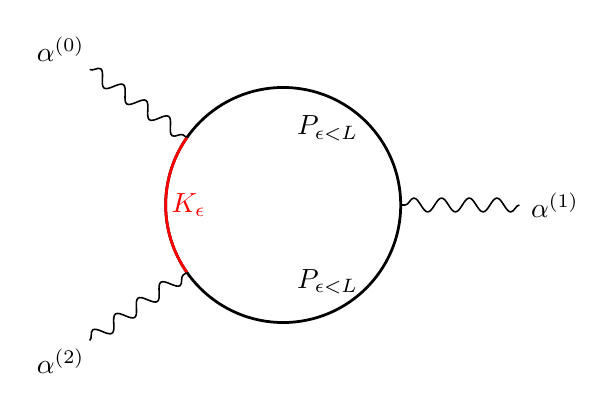
\begin{tikzpicture}[line width=.2mm, scale=1.5]

%\pgfmathsetmacro{\ex}{0}
%\pgfmathsetmacro{\ey}{1}

%\draw (\ex,\ey) ++(45:.8) arc (45:-45:.8);

		\draw[fill=black] (0,0) circle (1cm);
		%\draw[fill=red] (0,0) arc (145:215:1);
		\draw[fill=white] (0,0) circle (0.99cm);
		\draw[line width=0.35mm,red] ++(145:0.995) arc (145:215:0.995);
		%\draw[red] (0,0) arc (30:60:3);

		\draw[vector](145:2) -- (145:1);
		\node at (145:2.3) {$\alpha^{(0)}$};
			%\node at (145:0.85) {$v_0$};
		\node at (60:0.75) {$P_{\epsilon<L}$};
		\node at (-60:0.75) {$P_{\epsilon<L}$};
		\draw[vector](215:2) -- (215:1cm);
		\node at (215:2.3) {$\alpha^{(2)}$};
			%\node at (215:0.85) {$v_{d}$};
		\node[red] at (180:0.8) {$K_\epsilon$};
		\draw[vector](0:2) -- (0:1);
		\node at (0:2.3) {$\alpha^{(1)}$};
			%\node at (35:0.85) {$v_{\alpha}$};
		%\node at (0:0.8) {$P_{\epsilon<L}$};
		%\node at (270:0.8) {$P_{\epsilon<L}$};
	    	\clip (0,0) circle (1cm);
\end{tikzpicture}
\caption{The diagram representing the weight $W_{\Gamma, e}(P_{\epsilon<L}, K_\epsilon, I^\fg)$ in the case $d=2$. 
On the black internal edges are we place the propagator $P_{\epsilon < L}$ of the $\beta\gamma$ system. 
On the red edge labeled by $e$ we place the heat kernel $K_\epsilon$.
The external edges are labeled by elements $\alpha^{(i)} \in \Omega^{0,*}_c(\CC^2)$.}
\label{fig:liewheel}
\end{center}
\end{figure}

In particular, there is no obstruction to having an {\em action} by $\sG$, only an obstruction to having an {\em inner action}. 
Concretely, the external edges of any closed wheel occurring in the expansion of the anomaly must be labeled by $\sG$. 
As an immediate consequence we have the following.

\begin{lem}
The effective family $\{I^{\fg}[L]\}$ defines a one-loop exact $\sG$-equivariant quantum field theory.
In other words, it satisfies the $\sG$-equivariant quantum master equation modulo functionals purely of the background fields $\sG$. 
\end{lem}

It follows that the anomaly $\{\Theta[L]\}$ measures the obstruction to $\{I^\fg[L]\}$ to defining an {\em inner} action. 

%\begin{lem} 
%The one-loop effective family $\{I^\fg[L]\}$ 
%\[
%I^\fg [L] = \lim_{\epsilon \to 0} W(P_{\epsilon < L}, I^\fg) \mod \hbar^2
%\]
%is well-defined and satisfies the equivariant quantum master equation modulo $\cloc^*(\sG)[[\hbar]]$. 
%\end{lem}
%
%Working modulo $\hbar^2$ Lemma \ref{lem: inner action} implies that the anomaly to $\{I^{\fg}[L]\}$ to satisfying the quantum master equation modulo $\hbar^2$ is an element 
%\[
%\Theta_V \in \hbar \cloc^*(\sG) .
%\]
%The next subsection is devoted to an explicit calculation of this anomaly using Feynman diagrams. 

\subsubsection{The anomaly calculation}

We now perform the main technical calculation of the anomaly cocycle.

\begin{prop}\label{prop: inner anomaly}
The $L\to 0$ limit of the anomaly cocycle $\Theta = \lim_{L \to 0} \Theta_V[L]  \in \cloc^*(\sG)$ is of the form
\[
\Theta_V = C \cdot J_{\CC^d}(\ch_{d+1}^\fg (V)),
\]
where $\ch_{d+1}^\fg(V) \in \Sym^{d+1}(\fg^*)^\fg$ and where $J_{\CC^d} : \Sym^{d+1}(\fg^*)^\fg \to \cloc^*(\sG)$ is the map of Lemma \ref{prop j map} and where $C$ some constant only depending on the dimension $d$. 
\end{prop}

To compute the anomaly we refer to the following result about the expression for the anomaly cocycle in terms of the Feynman diagram expansion.
As a direct corollary of our general characterization of chiral anomalies, Lemma \ref{lem: chiral anomaly}, we have the following result.

\begin{lem}\label{lem: g anomaly}
The limit $\Theta_{V} := \lim_{L \to 0} \Theta_{V}[L]$ exists and 
is an element of degree one in $\clie^*(\Vect,\Cloc^*(\fg_n^\CC))$. 
Moreover, it is given by
\[
\Theta_V = \lim_{\epsilon \to 0} \sum_{\substack{\Gamma \in (d+1)\text{\rm -vertex wheels}\\ e \in {\rm Edge}(\Gamma)}} W_{\Gamma,e}(P_{\epsilon<1}, K_\epsilon,
I^{\rm \fg}[\epsilon]),
\]
where the sum is over wheels $\Gamma$ with $(d+1)$ vertices and a distinguished inner edge $e$.
\end{lem}

%Part of the data of a free theory is a gauge fixing condition $Q^{GF}$. 
%This is an operation on fields of cohomological degree $-1$ and enables us to fix the propagator uniquely. 
%For the $\beta\gamma$ system on $\CC^d$ with values in the vector space $V$ the gauge fixing operator we choose is 
%\[
%Q^{GF} = \dbar^* \tensor \id_V = \pm \sum_i \frac{\partial}{\partial z_i} \frac{\partial}{\partial (\d \zbar_i)} \tensor \id_V .
%\]

%The propagator with UV-IR cutoff $\epsilon,L$ is equal to
%\[
%P_{\epsilon, L} (z, w) = \int_{t = \epsilon}^L \dbar^* K_t(z,w)\d t .
%\]
%Here, 
%\[
%K_t (z,w) = k_t(z,w) \Omega(z,w) (\id_V \tensor 1 + 1 \tensor \id_{V^*})
%\]
%where $k_t$ the heat kernel for the Dolbeault Laplacian $\dbar^* \dbar + \dbar \dbar^*$ acting on smooth functions on $\CC^d$, $\Omega(z,w)$ is a constant coefficient differential form on~$\CC^d_z \times \CC^d_w$ satisfying
%\[
%\int_{z \in \CC^d} \phi(z) \wedge \Omega(z,w) = \pm \phi(w),
%\]
%and $\id_V , \id_{V^*} \in \Sym^2(V \oplus V^*)$ represent the identity maps $V \to V$, $V^* \to V^*$. 
%Explicitly, if we choose a basis $\{e_a\}$ for $V$ with dual basis $\{e_a^*\}$ we have the following formula for $K_t(z,w)$: 
%\[
%K_t(z,w) = \frac{1}{(4 \pi t)^d} e^{-|z-w|^2/ t} \left((\d^d z - \d^d w) \wedge \prod_{i} (\d \zbar_i - \d \Bar{w}_i) \right) \left(\sum_{a = 1}^{\dim V} (e_a \tensor e_a^* + e_a^* \tensor e_a) \right).
%\]

%Now, we are ready to apply Lemma \ref{lem anomaly} to compute the anomaly cocycle. 
%The fact that the limit of $W(P_{\epsilon,L}, I^{\sL})$ as $\epsilon \to 0$ exists is technical and left in the appendix. 
%We provide an explicit analysis of the sum of the Feynman weights corresponding to wheels.
%We find that the sum reduces to evaluating the weight of a single wheel with $d+1$ vertices. 

%Fix $k \geq 1$ to be the number of vertices of the wheel $\Gamma$. 
%By differential form type reasons, the wheels with number of vertices $k \leq d$ vanish identically. 
%To see this, note that the integral computing the Feynman weight is an integral over $\CC^{dk}$. 
%Each propagator contributes a differential form of Dolbeault type $(d, d-1)$.
%The heat kernel contributes a differential form of type $(d,d)$. 
%Thus, in total the internal edges contribute a differential form of type 
%\[
%(kd, (k-1)(d-1) + d) = (kd, (k-1)d + 1).
%\]
%Now, t	he anomaly is a cocycle of $\sL$ of cohomological degree $+1$.
%\brian{finish}
%
%The reason that the wheels of valency $k > d+1$ vanish is more subtle, and relies on analytic bounds of the integral computing the weight. 
%We provide this argument in the appendix. 

The lemma implies that we only need to consider the wheel with $d+1$ vertices. 
Each trivalent vertex is labeled by both an analytic factor and Lie algebraic factor. 
The Lie algebraic part of each vertex can be thought of as the defining map of the representation $\rho : \fg \to {\rm End}(V)$. 
The diagrammitcs of the wheel amounts to taking the trace of the symmetric $(d+1)$st power of this Lie algebra factor. 
Thus, the Lie algebraic factor of the weight of the wheel is the $(d+1)$st component of the character of the representation
\[
{\rm ch}_{d+1}^\fg(V) = \frac{1}{(d+1)!} {\rm Tr}\left(\rho(X)^{d+1}\right) \in \Sym^{d+1}(\fg^*) .
\]

To finish the calculation we must compute the analytic weight of the wheel with $d+1$ vertices. 
Recall, our goal is to identify the anomaly $\Theta$ with the image of ${\rm ch}_{d+1}^\fg(V)$ under the map
\[
J : \Sym^{d+1}(\fg^*)^\fg \to \cloc^*(\Omega^{0,*}(\CC^d)\tensor \fg)
\]
that sends an element $\theta$ to the local functional $\int \theta(\alpha \partial \alpha \cdots \partial \alpha)$. 
We have just seen that the Lie algebra factor in local functional representing the anomaly agrees with the $(d+1)$st Chern character. 
Thus, to finish we must show the following.

\begin{lem} 
As a functional on the abelian dg Lie algebra $\Omega^{0,*}(\CC^d)$, the analytic factor of the weight $\lim_{L\to 0} \lim_{\epsilon \to 0} W_{\Gamma, e} (P_{\epsilon < L}, K_\epsilon, I^\fg)$ is equal to a multiple of the local functional
\[
\int \alpha \partial \alpha \cdots \partial \alpha \in \cloc^*(\Omega^{0,*}(\CC^d)) .
\]
\end{lem}

\begin{proof}

Let's fix some notation. 
We enumerate the vertices by integers $a = 0,\ldots, d$. 
Label the coordinate at the $i$th vertex by $z^{(a)} = (z_1^{(a)}, \ldots, z_d^{(a)})$. 
The incoming edges of the wheel will be denoted by homogeneous Dolbeault forms 
\[
\alpha^{(a)} = \sum_{J} A^{(a)}_J \d \zbar_J^{(a)} \in \Omega_c^{0,*}(\CC^d) .
\]
where the sum is over the multiindex $J = (j_1,\ldots, j_k)$ where $j_a = 1,\ldots, d$ and $(0,k)$ is the homogenous Dolbeault form type. 
For instance, if $\alpha$ is a $(0,2)$ form we would write
\[
\alpha = \sum_{j_1 < j_2} A_{(j_1,j_2)} \d \zbar_{j_1} \d\zbar_{j_2} .
\]
Denote the functional obtained as the $\epsilon \to 0$ weight of the wheel with $(d+1)$ vertices from Lemma \ref{lem: g anomaly} by $W_L$.
The $L\to 0$ limit of $W_L$ is the local functional representing the one-loop anomaly $\Theta$. 

The weight has the form
\[
W_L(\alpha^{(0)},\ldots,\alpha^{(d)}) = \pm \lim_{\epsilon \to 0} \int_{\CC^{d(d+1)}} \left(\alpha^{(0)}(z^{(0)}) \cdots \alpha^{(d)}(z^{(d)}) \right) K_\epsilon(z^{(0)},z^{(d)}) \prod_{a =1}^d P_{\epsilon,L} (z^{(a-1)}, z^{(a)}) .
\]
We introduce coordinates
\begin{align*}
w^{(0)} & = z^{(0)} \\
w^{(a)} & = z^{(a)} - z^{(a-1)} \;\;\; 1 \leq a \leq d .
\end{align*}
The heat kernel and propagator part of the integral is of the form
\[
\begin{array}{ccl}
\displaystyle
K_\epsilon(w^{(0)},w^{(d)}) \prod_{a =1}^d P_{\epsilon,L} (w^{(a-1)}, w^{(a)}) & = & \displaystyle \frac{1}{(4 \pi \epsilon)^d} \int_{t_1,\ldots,t_d = \epsilon}^L \frac{\d t_1 \cdots \d t_d}{(4 \pi t_1)^d \cdots (4 \pi t_d)^d} \frac{1}{t_1\cdots t_d}  \\ & & \displaystyle \times \d^d w^{(0)} \prod_{i=1}^d (\d \Bar{w}^{(1)}_i + \cdots + \d \Bar{w}^{(d)}_i) \prod_{a = 1}^d \d^d w^{(a)} \left(\sum_{i = 1}^d \Bar{w}_i^{(a)} \prod_{j \ne i} \d \Bar{w}_{j}^{(a)}\right)
\\ & & \displaystyle \times e^{-\sum_{a,b = 1}^d M_{a b} w^{(a)} \cdot \Bar{w}^{(b)}} .
\end{array}
\]
Here, $M_{ab}$ is the $d \times d$ square matrix satisfying
\[
\sum_{a,b = 1}^d M_{a b} w^{(a)} \cdot \Bar{w}^{(b)} = |\sum_{a = 1}^d w^{(a)} |^2 / \epsilon + \sum_{a = 1}^d |w^{(a)}|^2 / t_a .
\]
Note that
\[
\prod_{i=1}^d (\d \Bar{w}^{(1)}_i + \cdots + \d \Bar{w}^{(d)}_i) \prod_{a = 1}^d \left(\sum_{i = 1}^d \Bar{w}_i^{(a)} \prod_{j \ne i} \d \Bar{w}_{j}^{(a)}\right) = \left( \sum_{i_1,\ldots i_d} \epsilon_{i_1\cdots i_d} \prod_{a=1}^d \Bar{w}^{(a)}_{i_a}\right) \prod_{a=1}^d \d^d \Bar{w}^{(a)} .
\]
In particular, only the $\d w_i^{(0)}$ components of $\alpha^{(0)} \cdots \alpha^{(d)}$ can contribute to the weight.

For some compactly supported function $\Phi$ we can write the weight as
\[
\begin{array}{ccl}
W (\alpha^{(0)}, \ldots, \alpha^{(d)}) & = & \lim_{\epsilon \to 0} \displaystyle \int_{\CC^{d(d+1)}} \left(\prod_{a = 0}^{d} \d^d w^{(a)} \d^d \Bar{w}^{(a)}\right) \Phi \\ & \times & \displaystyle \frac{1}{(4 \pi \epsilon)^d} \int_{t_1,\ldots,t_d = \epsilon}^L \frac{\d t_1 \cdots \d t_d}{(4 \pi t_1)^d \cdots (4 \pi t_d)^d} \frac{1}{t_1\cdots t_d} \sum_{i_1,\ldots, i_d} \epsilon_{i_1\cdots i_d} \Bar{w}_{i_1}^{(1)} \cdots \Bar{w}_{i_d}^{(d)} e^{-\sum_{a,b = 1}^d M_{a b} w^{(a)} \cdot \Bar{w}^{(b)}} 
\end{array}
\]

Applying Wick's lemma in the variables $w^{(1)}, \ldots, w^{(d)}$, together with some elementary analytic bounds, we find that the weight above becomes to the following integral over $\CC^d$
\[
f(L) \int_{w^{(0)} \in \CC^d}  \d^d w^{(0)} \d^d \Bar{w}^{(0)} \sum_{i_1,\ldots, i_d} \epsilon_{i_1\cdots i_d}  
\left(\frac{\partial}{\partial w_{i_1}^{(1)}} \cdots \frac{\partial}{\partial w_{i_d}^{(d)}} \Phi\right)|_{w^{(1)}=\cdots=w^{(d)} = 0} 
\]
where
\[
f(L) = \lim_{\epsilon \to 0} \int_{t_1,\ldots,t_d = \epsilon}^L \frac{\epsilon}{(\epsilon + t_1 + \cdots + t_d)^{d+1}} \d^d t .
\]
In fact, $f(L)$ is independent of $L$ and is equal to some nonzero constant $C \ne 0$.
Finally, plugging in the forms $\alpha^{(0)}, \ldots, \alpha^{(d)}$, we observe that the integral over $w^{(0)} \in \CC^d$ simplifies to
\[
C \int_{\CC^d} \alpha^{(0)} \partial \alpha^{(1)} \cdots\partial \alpha^{(d)}
\]
as desired.
\end{proof}

This completes the proof of Proposition \ref{prop: inner anomaly}.

\subsection{Local to global}

In this section we finish the proof of our main result Theorem \ref{thm ggrr} by showing how our local calculation above implies the formula for the anomaly on a general compact affine manifold $X$.
By an complex affine manifold, we mean a quotient 
\[
q : U \subset \CC^d \to X
\]
of an open subset $U \subset \CC^d$ by a free and proper action of a discrete subgroup of the affine group $U(d) \ltimes \CC^d$. 
We consider affine manifolds that are also compact. 
To deduce our main theorem we will show that the theory and the anomaly above also exhibit equivariance for the affine group on $\CC^d$, thus it will descend to any affine manifold.

We have stated the main result for an arbitrary principal $G$-bundle $P$ on the affine manifold $X$. 
Suppose the discrete subgroup $\Gamma \leq U(d) \ltimes \CC^d$ defines the affine manifold $q : U \to X = U / \Gamma$ as above. 
Then, principal $G$-bundles on $X$ are equivalent to $\Gamma$-equivariant principal $G$-bundles on $U$. 

Let $\sE$ be an arbitrary elliptic complex on $X$, and suppose the Lie algebra $\fh$ acts on $\sE$. 
Since $X$ is compact, the cohomology $H^*(\sE(X))$ is finite dimensional.
It therefore makes sense to define the character of the action of $\fh$ on $H^*(\sE(X))$.
\beqn\label{superchar}
\chi_\sE : \fh \to \CC \;\; , \;\; M \in \fh \mapsto {\rm STr}_{H^*(\sE(X))} (M) .
\eeqn
Here, STr denotes the supertrace. 
The character factors through the determinant of the representation.
For the graded character above, we must use the superdeterminant which we denote by $\det (H^*(\sE(X)))$. 
Free BV quantization gives a natural field theoretic interpretation of this determinant.

\begin{prop}[\cite{CG2} Lemma 12.7.0.1] 
Let $\sE$ be any elliptic complex on a compact manifold $X$ and let $T^*[-1] \sE$ be the corresponding free BV theory given by the shifted cotangent bundle. 
Let $\Obs^\q_\sE$ be the factorization algebra of quantum observables of this theory.
Then, there is an isomorphism
\[
H^* \left(\Obs^\q_{\sE}(X) \right) \cong \det H^*(\sE(X)) [n]
\]
where $n$ is the Euler characteristic of $\sE(X)$ modulo $2$. 
\end{prop}

\begin{rmk}
In \cite{GwilliamHaugseng} they prove that an abstracted version of linear BV quantization behaves like a determinant over formal moduli problems.
An immediate consequence is that given a classical theory with an action of a Lie algebra $\fg$, the BV quantization as we consider produces a line bundle over the moduli space $B \fg$. 
Our calculation of the obstruction produces a calculation in terms of Feynman diagrams of the first Chern class of this line bundle. 
\end{rmk}
 
Notice that the classical free theory $\sE_V$ is equivariant for the affine group $U(d) \ltimes \CC^d$.
Thus, it defines a classical theory on any affine manifold $X$.
This theory is free and of the form
\[
\sE_V (X) = T^*[-1] (\Omega^{0,*}(X , V))
\]
where $T^*[-1]$ denotes the shifted cotangent bundle.
Thus, the global quantum observables satisfy
\beqn\label{quantum obs}
H^*(\Obs^\q_{V}(X)) = \det \left(H^*(X, \sO^{hol}) \tensor V \right)
\eeqn
 
%Similarly, the functional $I^\fg$ is equivariant for the affine group, so that it also descents to a functional on $X$.
%Thus, the Noether current $I^\fg$ defines a \brian{finish}

In Section \ref{sec: classical g equiv} we have showed how the classical theory $\sE_{V}$ has an an action by the local Lie algebra $\sG_X$.
This arose from an action of $\sG(X) = \Omega^{0,*}(X, \fg)$ on the elliptic complex $\Omega^{0,*}(X, V)$. 
At the level of cohomology we have an action of $H^*(\sG(X))$ on $H^*(\Omega^{0,*}(X, V))$ and hence a character $\chi_{V}$ as in Equation (\ref{superchar}) which is an element in $H^*_{red}(\sG(X))$. 

The local Lie algebra cohomology of any local Lie algebra embeds inside its ordinary (reduced) Lie algebra cohomology of global sections $\cloc^*(\sL(X)) \subset \cred^*(\sL(X))$. 
The character (\ref{superchar}) is an element in $H_{red}^*(\sL(X))$.
As an immediate corollary of \cite{CG2} Theorem 12.6.0.1 we have the following relationship between the anomaly cocycle and the character.

\begin{prop}\label{inner char}
Suppose $\sL$ is a local Lie algebra that acts on the elliptic complex $\sE$ on a compact manifold $X$.
Let $\Theta_\sE \in \cloc^*(\sL)$ be the local cocycle measuring the failure to satisfy the $\sL$-equivariant classical master equation (that is, the obstruction to having an inner action).
Then, its global cohomology class satisfies $[\Theta_\sE (X)] = \chi_{\sE} \in \cred^*(\sL(X))$ where $\chi_\sE$ is the trace of the action of $H^*(\sL(X))$ on $H^*(\sE(X))$. 
\end{prop}

%\begin{proof}
%A version of this is proved in Section 7 of \cite{GwilliamThesis}, but we will sketch the proof here.
%\end{proof}

For the case of $\sL = \sG_X$ we have an embedding of cochain complexes
\[
\cloc^*(\sG(X)) \hookrightarrow \cred^*(\sG(X)) = \cred^*(\Omega^{0,*}(X) \tensor \fg) .
\]
By Kodaira-Spencer theory have already seen that the global sections of the local Lie algebra $\sG(X)$ is a model for the formal neighborhood of the trivial $G$-bundle inside of $G$-bundles. 
In particular, the $\sG(X)$-module of quantum observables defines a line bundle $\int_X \Obs^\q_{\sE_V}$ over this formal neighborhood.
Its character as a $\sG(X)$-module is identified with the first Chern class of the corresponding line bundle $\chi_\sE(\Obs^\q_{V}(X)) = c_1(\int_X \Obs^\q_{V})$. 

Now, notice that the one-loop quantization we constructed in the previous section, as well as the anomaly cocycle $\Theta_V \in \cloc^*(\sG_{\CC^d})$ are equivariant for the group $U(d) \ltimes \CC^d$. 
Thus, they descend to the global sections of $\cloc^*(\sG_X)$ for any affine manifold $X$.
Explicitly, if $\Gamma\subset U(d) \ltimes \CC^d$ is the discrete subgroup such that $X = U / \Gamma$ where $U \subset \CC^d$, then under the isomorphism 
\[
\cloc^*(\sG(X)) \cong \cloc^*(\sG(U))^\Gamma
\]
we have $\Theta_V(X) \leftrightarrow \Theta_V(U)$.

Further, we have an identification
\[
\cred^*(\Omega^{0,*}(X) \tensor \fg) = \sO_{red}\left({\rm Bun}_G(X)^{\wedge}_{triv}\right) \cong  \Omega^1_{cl} \left({\rm Bun}_G(X)^{\wedge}_{triv}\right) 
\]
where we have used the equivalence of reduced functions and closed one-forms which makes sense on any formal moduli space.
At the level of $H^1$ we have the composition composition
\beqn\label{cohbung}
\Sym^{d+1}(\fg^*)^\fg \xto{J^X} H^1_{\rm loc} (\sG(X)) \to H^1(\Omega^1_{cl}\left({\rm Bun}_G(X)^{\wedge}_{triv}\right) .
\eeqn
As a corollary of Proposition \ref{inner char} and our calculation of the local anomaly cocycle we see that the image of $\ch_{d+1}^\fg(V)$ is equal to $[\Theta_V(X)] = [c_1(\int_X \Obs^\q_V)]$. 

The same holds when we work around any holomorphic principal bundle $P$ on $X$, so that we have an embedding of cochain complexes
\[
\cloc^*(\sAd(P)(X)) \hookrightarrow  \Omega^1_{cl} \left({\rm Bun}_G(X)^{\wedge}_{P}\right) . 
\]
which determines a composition
\beqn\label{cohbung}
\Sym^{d+1}(\fg^*)^\fg \xto{J_P^X} H^1_{\rm loc} (\sAd(P)(X)) \to H^1(\Omega^1_{cl}\left({\rm Bun}_G(X)^{\wedge}_{P}\right) .
\eeqn
Since every principal $G$-bundle $P$ on $X$ is trivial when we pull it back to $U\subset \CC^d$, the above local anomaly calculation proves that $[c_1(\int_X \Obs^\q_{P,V})] = C \ch_{d+1}^\fg (V)$ in this case as well.
This completes the proof of Theorem \ref{thm ggrr}. 

\subsection{A module for the higher Kac-Moody}

The last part of this section we diverge to deduce a consequence of the quantum Noether theorem using our analysis above by exhibiting a module for the higher affine algebras from the previous section. 
For convenience, we fix the trivial $\fg$-bundle $P = {\rm triv}$ so that $\sAd(P) = \sG_X$.

On any manifold $X$, the quantum Noether theorem, Theorem 12.1.0.1 of \cite{CG2}, provides a map of factorization algebras
\[
\Phi_X : \UU_\alpha (\sG_X) \to \Obs^\q_{V} ,
\]
for some $\alpha \in H^1_{\rm loc}(\sG_X)$.
The factorization algebra $\Obs^\q_V$ is the quantum observables of the $\beta\gamma$ system on $X$ with values in the $\fg$-module $V$. 
This is a free field theory, thus the above map has the flavor of a {\em free field realization} of the Kac-Moody factorization algebra.
In particular when $X = \CC^d$, or any affine manifold, the calculation above shows that there is a map of factorization algebras
\[
\Phi_{\CC^d} : \UU_{\ch_{d+1}(V)} (\sG_{\CC^d}) \to \Obs^\q_{V} .
\]

Next, consider the case $X = \CC^d \setminus  \{0\}$. 
By functoriality of pushforwards, the quantum Noether theorem produces a map of one-dimensional factorization algebras
\[
\rho_* \Phi : \rho_* \UU_{\ch_{d+1}(V)} (\sG_{\CC^d \setminus \{0\}}) \to \rho_* \Obs^\q_{V} .
\]
We have exhibited a locally constant dense subfactorization algebra $\sF^{lc}_{1d}$ of $\rho_* \UU_\alpha (\sG_X)$ which is equivalent, as an $E_1$-algebra, to $U \Hat{\fg}_{d, \ch_{d+1}(V)}$. 
Similarly, in Section \ref{sec: sphere ops} we have shown that there is a locally constant dense subfactorization algebra that is equivalent to the dg algebra $\sA_V$. 

The map $\rho_* \Phi$ restricts to these dense subfactorization algebras and so defines a map of $E_1$ algebras
\[
\rho_* \Phi : U \Hat{\fg}_{d, \ch_{d+1}(V)}\to \sA_V .
\]
Also, in Section \ref{sec: disk module} we have shown how the disk operators $\sV_V$ form a module, through the factorization product, for the dg algebra $\sA_V$. 
This is essentially the Fock module of the algebra $\sA_V$, thus we should view the above map $\rho_*\Phi$ as being a higher dimensional analog of the ``free field realization" for the higher dimensional affine algebras. 

Further, by induction along the map $\rho_* \Phi$, we obtain the following.

\begin{prop}
The map $\rho_*\Phi$ endows the space $\sV_V$ with the structure of a module over the $E_1$-algebra $U \Hat{\fg}_{d, \ch_{d+1}(V)}$.
Equivalently, $\sV_V$ is an $A_\infty$-module for $U \Hat{\fg}_{d, \ch_{d+1}(V)}$. 
\end{prop}

The module $\sV_V$ is the prototype for a higher dimensional version of the vacuum Verma module for ordinary affine algebras. 
It is enticing to construct the higher excitation Verma modules as dg modules for the higher affine algebras we've considered in this thesis.
We do not do that here, but hope to return to it in future work.

\end{document}